\section{Regression analysis on mean annual SIE}

Before doing any spatial analysis we will take a moment to apply the regression analysis to the mean value of SIE over our time period. The simplest and first step we take is to plot the annual values of SIE against each of the indices we are investigating.
\begin{figure}[H]
    \centering
    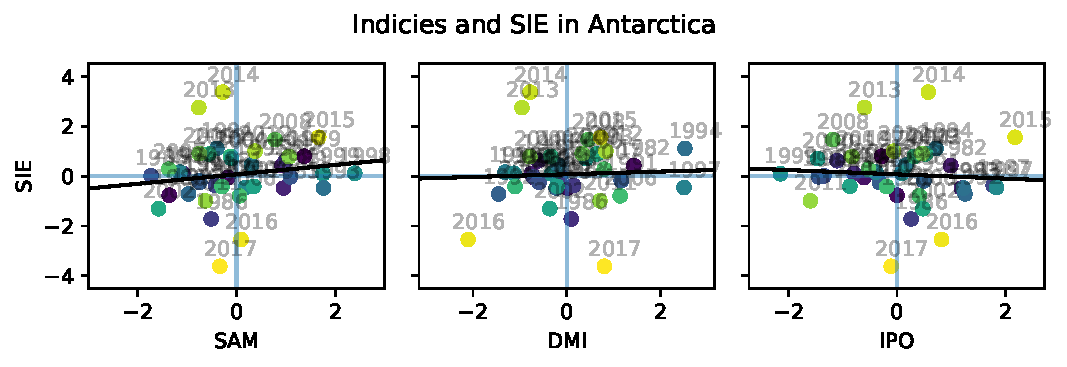
\includegraphics[width=\linewidth]{Images_3.0/regressions/scatter_anomalous_n1_annually_detrended_1979_2018.pdf}
    \caption{Regression of SIC for each of the indices for 1979 to 2018.}
    \label{fig:scatter_anomalous_n1_annually_1979_2018}
\end{figure}
We note that these results are consistent with what we found in the correlation analysis. SAM has a positive relationship with SIE, while DMI has a very weak positive relationship and IPO has a weak negative relationship. This doesn't give us new information, however the consistency indicates that the regression analysis provides somewhat reliable results results. Plotting the same thing for before and after December 2001 when IPO is in negative and positive phases respectively gives the following plots.

\begin{figure}[H]
    \begin{subfigure}{\linewidth}
    \centering
    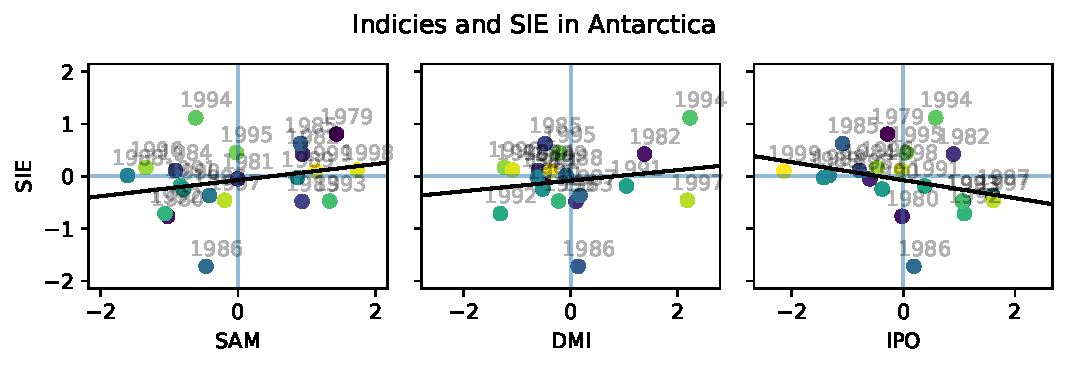
\includegraphics[width=\linewidth]{Images_3.0/regressions/scatter_anomalous_n1_annually_detrended_1979_2000.pdf}
    \caption{Regression of SIC for each of the indices for 1979 to 2000.}
    \label{fig:scatter_anomalous_n1_annually_1979_2000}
    \end{subfigure}
    
    \begin{subfigure}{\linewidth}
    \centering
    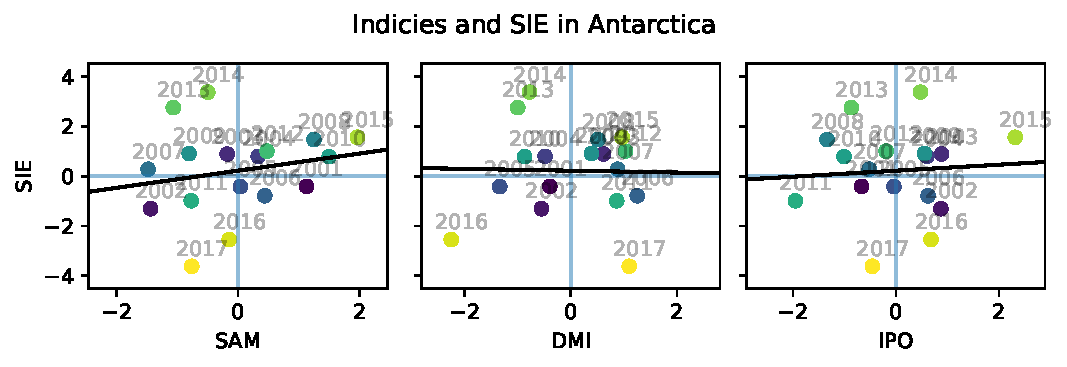
\includegraphics[width=\linewidth]{Images_3.0/regressions/scatter_anomalous_n1_annually_detrended_2001_2018.pdf}
    \caption{Regression of SIC for each of the indices for 2001 to 2018.}
    \label{fig:scatter_anomalous_n1_annually_2001_2018}
    \end{subfigure}
    \caption{Regressions for SIE for the different time periods in our dataset.}
\end{figure}
Here we can see that there is little change for the SAM relationship with SIE whereas the relationship between IPO experiences a significant change, shifting from a negative relationship before 2001 and a positive relationship after 2001. DMI has a positive relationship before 2001 and a weak negative relationship after 2001.

\subsection{Regression analysis on mean monthly SIE}
We have the same plots for the monthly version of the data.
\begin{figure}[H]
    \begin{subfigure}{\linewidth}
    \centering
    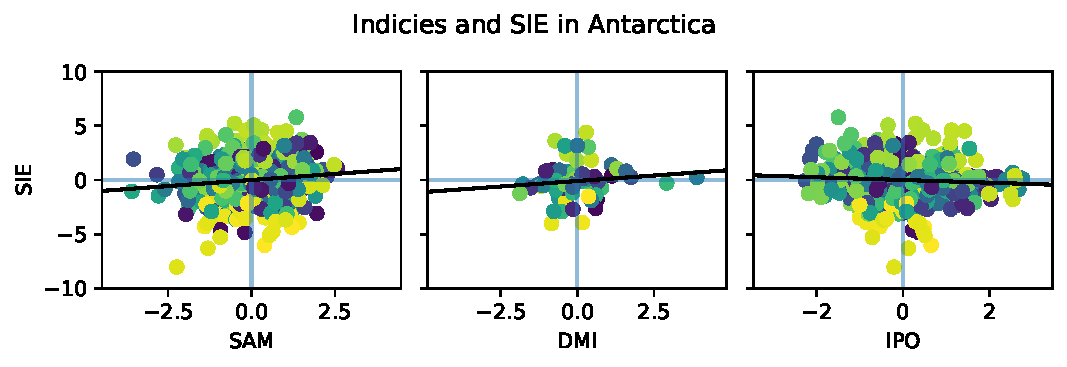
\includegraphics[width=\linewidth]{Images_3.0/regressions/scatter_anomalous_n1_monthly_detrended_1979_2018.pdf}
    \caption{Regression of SIC for each of the indices for 1979 to 2018.}
    \label{fig:scatter_anomalous_n1_annually_1979_2018}
    \end{subfigure}
    
    \begin{subfigure}{\linewidth}
    \centering
    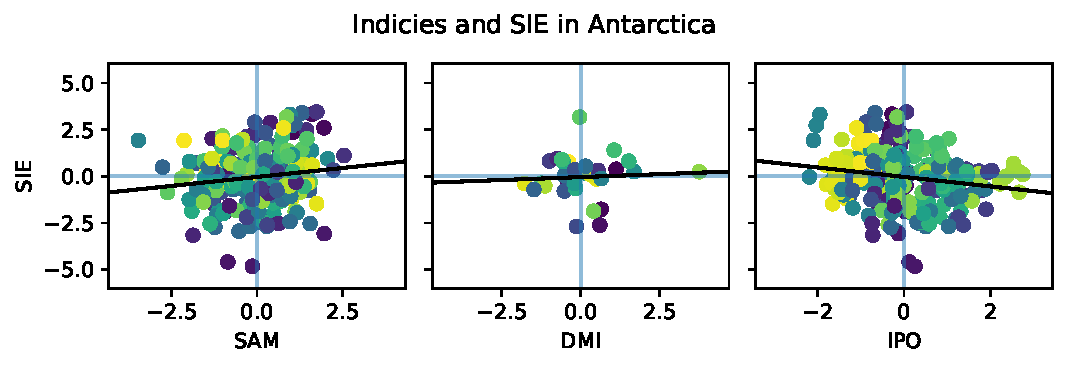
\includegraphics[width=\linewidth]{Images_3.0/regressions/scatter_anomalous_n1_monthly_detrended_1979_2000.pdf}
    \caption{Regression of SIC for each of the indices for 1979 to 2000.}
    \label{fig:scatter_anomalous_n1_annually_1979_2000}
    \end{subfigure}
    
    \begin{subfigure}{\linewidth}
    \centering
    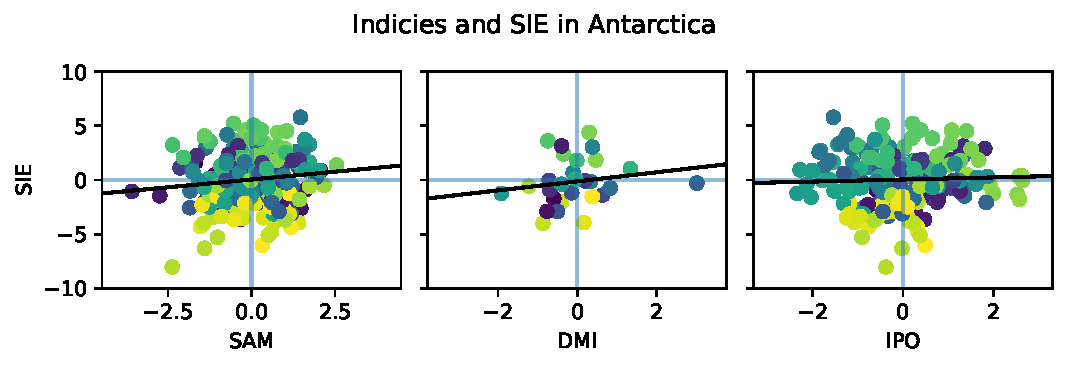
\includegraphics[width=\linewidth]{Images_3.0/regressions/scatter_anomalous_n1_monthly_detrended_2001_2018.pdf}
    \caption{Regression of SIC for each of the indices for 2001 to 2018.}
    \label{fig:scatter_anomalous_n1_annually_2001_2018}
    \end{subfigure}
    \caption[Regressions for SIE for the different time periods in our dataset.]{Regressions for SIE for the different time periods in our dataset. The colour represents years with blue being early years and yellow representing latter years.}
\end{figure}
The main difference in these plots when compared with the annual averages is the relationship between SIE and IPO and DMI after 2001. DMI has a positive relationship for the monthly means whereas it has a negative relationship for the annual means. IPO has a weaker relationship for the monthly means than the annual means.
\section{Applying the regression model}
After doing this initial analysis we can apply the regression analysis using the model:
$$
\text{SIE} = a\times\text{SAM} + b\times\text{DMI} + c \times\text{IPO} + d
$$
We can look at the quality of this fit by plotting this model prediction and the actual SIE time-series against each other.
\begin{figure}[H]
    % \begin{subfigure}{\linewidth}
    \centering
    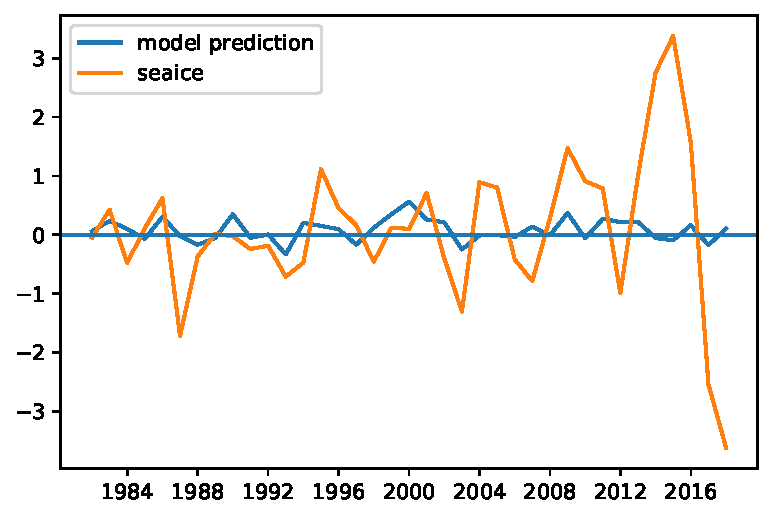
\includegraphics{Images_3.0/regressions/multivariate_model_anomalous_n1_annually_detrended_1979_2018.pdf}
    \caption{Fitted model for SIE detrended and averaged annually from 1979 to 2018.}
    \label{fig:multivariate_model_anomalous_n1_annually_detrended_1979_2018}
    % \end{subfigure}
\end{figure}
This doesn't seem to be a good fitting. This isn't surprising for a number of reasons. Firstly the regressions done on each individual index were each relatively weak and so we don't expect a strong fitting when done in concert. Additionally the system we are looking at is intrinsically complex and probably nonlinear, which leads to a bad fitting with a linear model. Additionally because we are only looking at the mean value for SIE this plot will have lost information because the indices probably affect different spatial regions of SIC in different ways. This is something we will explore further.
\begin{figure}[H]
    \begin{subfigure}{\linewidth}
    \centering
    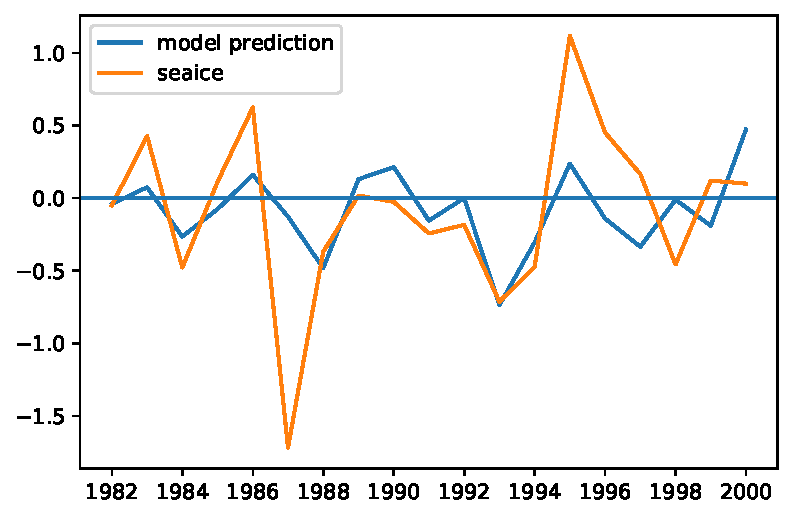
\includegraphics{Images_3.0/regressions/multivariate_model_anomalous_n1_annually_detrended_1979_2000.pdf}
    \caption{Fitted model for SIE detrended and averaged annually from 1979 to 2000.}
    \label{fig:multivariate_model_anomalous_n1_annually_detrended_1979_2000}
    \end{subfigure}
    
    \begin{subfigure}{\linewidth}
    \centering
    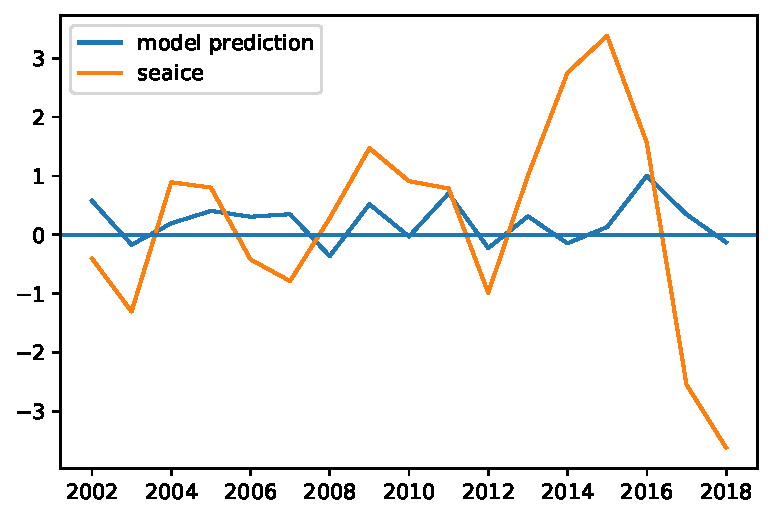
\includegraphics{Images_3.0/regressions/multivariate_model_anomalous_n1_annually_detrended_2001_2018.pdf}
    \caption{Fitted model for SIE detrended and averaged annually from 2001 to 2018.}
    \label{fig:multivariate_model_anomalous_n1_annually_detrended_2001_2018}
    \end{subfigure}
    \caption{Fitted model for SIE detrended and averaged annually. Before and after December 2000.}
\end{figure}

Likewise to looking at the entire time period, these plots are also demonstrating a bad fitting \textcolor{red}{put these in the same plot for easier comparison?}. For the same reasons as before this is unsurprising.
